\chapter{Umsetzung der Interaktion}
\label{Kap4}
\label{chap:Kap4}
Dieses Kapitel beschreibt Konzepte für die im vorangegangen Kapitel identifizierten Teilsysteme. Diese Konzepte beziehen sich zu einem großen Teil auf \acs{iOS} Frameworks, mit denen die Demonstrator Applikation entwickelt wurde. Aus diesem Grund werden diese Frameworks einleitend in Abschnitt \ref{sec:iOSFrameworks} beschrieben. Darauf folgt in Abschnitt \ref{sec:BumpErkennung} ein Konzept zur Erkennung von Bumps, in Abschnitt \ref{sec:Ident} werden Konzepte zur Identifizierung der Endgeräte beschrieben und in Abschnitt \ref{sec:Austausch} Konzepte zum Datenaustausch zwischen den Endgeräten.

\section{Grundlagen zu iOS Frameworks}
\label{sec:iOSFrameworks}
\acs{iOS} bietet durch Frameworks Zugang zu verschiedenen Technologien. Im folgenden wird die grundlegende Funktionsweise von drei Frameworks beschrieben, die zur Umsetzung der Bump-Interaktion genutzt wurden.

\subsection{Core Motion Framework}
\label{subsec:coreMotion}
Das Core Motion Framework bietet Applikationen Zugang zu Sensordaten die durch die Gerätehardware erfasst werden. Die Klasse \textit{CMMotionManager} ist die zentrale Anlaufstelle für den Zugriff auf alle Sensoren die Daten durch die Bewegung des Endgeräts erzeugen. Somit bietet sie auch Zugang zu den Daten des Beschleunigungssensors. Wird dieser konfiguriert ist die Variable \textit{accelerometerUpdateInterval} sehr wichtig.  

\begin{description}
  \item \textcolor{type}{var} \noindent\hspace*{1mm} accelerometerUpdateInterval: \textcolor{parameter}{NSTimeInterval}
        \\[2mm]
\end{description}

Die Variable legt das Intervall in Sekunden fest, in denen die Accelerometer-Daten aktualisiert werden und sollte dem Anwendungskontext entsprechend gewählt werden. Um Entwicklern Unterstützung zu bieten, die richtige Wahl zu treffen, bietet Apple die folgenden Empfehlungen \cite{AppleAccelerometer:Online}.

\begin{table}[H]
\begin{tabular}{|p{0.3\linewidth}|p{0.65\linewidth}|}
\hline
\cellcolor[HTML]{C0C0C0}Frequenz (Hz) & \cellcolor[HTML]{C0C0C0} Nutzung                                                                                                                                                                   \\ \hline
10–20                & Geeignet um die Ausrichtung des Geräts festzustellen.                                                                                                         \\ \hline
\cellcolor[HTML]{EFEFEF}30–60                & \cellcolor[HTML]{EFEFEF} Geeignet für Spiele und andere Applikationen die Eingaben des Benutzers in Echtzeit verarbeiten müssen.
                                                                                  \\ \hline
70–100               & Geeignet für Applikationen die Hochfrequente Bewegungen (Schütteln, Stöße) feststellen müssen.  \\ \hline
\end{tabular}
\caption{Beschleunigungssensor Aktualisierungsintervall \cite{AppleAccelerometer:Online}}
\label{accelerometerInterval}
\end{table}

Um die Daten des Sensors abzufragen, wird die Funktion \textit{accelerationUpdated} genutzt. Es handelt sich dabei um eine Callback-Funktion, die im festgelegten Intervall aufgerufen wird \cite{AppleAccelerometer:Online}.
\begin{description}
  \item \textcolor{type}{func} accelerationUpdated(accelerometerData: \textcolor{parameter}{CMAccelerometerData!}, error: \textcolor{parameter}{NSError!}) -> \textcolor{parameter}{Void}
        \\[2mm]
\end{description}


\subsection{Core Location Framework}
\label{subsec:coreLocation}
Das Core Location Framework bietet Zugriff auf die Technologien \acs{GPS} und iBeacon, mit denen standortbasierte Dienste realisiert werden können. Die Funktionsweise dieser Technologien wurde bereits in den Abschnitten \ref{subsec:beacons} und \ref{subsec:GPS} beschrieben. Dieser Abschnitt beschreibt für die Implementierung relevante Klassen und Protokolle.

Die zentrale Anlaufstelle für Ortungsdienste ist die Klasse \textit{CLLocationManager} und das dazugehörige Protokoll \textit{CLLocationManagerDelegate}. Werden \acs{GPS} Standortdaten gesucht, sind diese, sobald Sie verfügbar sind, über die Delegate-Methode \textit{didUpdateLocations} verfügbar.

\begin{description}
  \item \textcolor{type}{func} locationManager(manager: \textcolor{parameter}{CLLocationManager!}, didUpdateLocations: \textcolor{parameter}{[AnyObject]!})
\end{description}

Wird nach iBeacons gesucht, wird die Delegate-Methode \textit{didRangeBeacons} aufgerufen. Diese liefert ein Array mit allen gefundenen Beacons in Empfangsreichweite. Die Beacons in diesem Array sind sortiert nach ihrer gemessenen Entfernung, beginnend mit dem Beacon das die kürzeste Entfernung aufweist.

\begin{description} 
  \item \textcolor{type}{func} locationManager(manager: \textcolor{parameter}{CLLocationManager!}, didRangeBeacons: \textcolor{parameter}{[CLBeacon]!}, inRegion: \textcolor{parameter}{ CLBeaconRegion!})
\end{description}

\subsection{Multipeer Connectivity Framework}
Mit dem Multipeer-Connectivity-Framwork können \acs{iOS} und \acs{MacOS} Geräte über \ac{WLAN} oder Bluetooth kommunizieren. Dabei nutzen die Endgeräte jene Kommunikationskanäle, die verfügbar sind. Sind sie Teil eines Infrastrukturnetzwerkes, können Sie darüber Daten austauschen. Ist keine Verbindung zu solch einem Netzwerk vorhanden, wird je nachdem, welche Technologie bei den Kommunikationspartnern aktiviert, ist eine Ad-Hoc Verbindung über Bluetooth oder \ac{WLAN} aufgebaut \cite{AppleMultipeer:Online}.

Das Framework operiert in zwei Phasen, der \textit{Discovery Phase} und der \textit{Session Phase}. Diese werden folgend beschrieben.

\subsubsection{Discovery Phase}
In der Discovery Phase können sich Endgeräte, die in Empfangsreichweite zueinander sind, gegenseitig entdecken und eine Verbindung miteinander aufbauen. Mit den Klassen \textit{MCNearbyServiceAdvertiser} und \textit{MCNearbyServiceBrowser} können die Geräte Dienste anbieten und suchen. Um einen \textit{Advertiser} oder einen \textit{Browser} zu initialisieren müssen eine \textit{MCPeerID} und ein \textit{serviceType} als Parameter übergeben werden. Während die \textit{peerID} jedes Peer identifiziert, handelt es sich beim serviceType um einen bis zu 15 Zeichen langen Bezeichner, der bei allen Peers, die sie sich gegenseitig entdecken möchten, übereinstimmen muss \cite{AppleMultipeer:Online}.

\begin{description}
  \item \textcolor{class}{class} MCNearbyServiceAdvertiser(peer: \textcolor{parameter}{MCPeerID!}, discoveryInfo: \textcolor{parameter}{[NSObject : AnyObject!]}, serviceType: \textcolor{parameter}{String!})
  \item  \textcolor{class}{class} MCNearbyServiceBrowser(peer: \textcolor{parameter}{MCPeerID!}, serviceType: \textcolor{parameter}{String!})
\end{description}

Zusätzlich zu peerId und serviceType verfügt der MCNearbyServiceAdvertiser noch den optionalen Paramter \textit{discoveryInfo}. Dabei handelt es sich um ein \textit{dictionary}, in dem zusätzliche Informationen vom Advertiser an den Browser übermittelt werden können. Ein dictionary ist ein Datentyp bei dem Daten (\textit{values}) eines bestimmten Typs ungeordnet gespeichert werden. Diese können durch einen einzigartigen Bezeichner, auch \textit{key} genannt, referenziert und gesucht werden \cite{AppleCollectionTypes:Online}. Key und value des dictionarys müssen String Objekte sein und dürfen zusammen eine Größe von 255 Bytes nicht überschreiten. Für optimale Performance sollte das gesamte dictionary nicht größer als 400 Bytes sein, damit es in einem einzelnen Bluetooth Datenpaket untergebracht werden kann \cite{AppleMCNearbyServiceAdvertiser:Online}.

\subsubsection{Advertising und Browsing}
Startet ein Peer das Advertisement, wird dieses Peer für alle Browser in Empfangsreichweite sichtbar und teilt diesen Peers die Bereitschaft zum Verbindungsaufbau mit. Advertiser in Empfangsreichweite werden dem Browser über die Delegate Methode \textit{foundPeer} des \textit{MCNearbyServiceBrowserDelegate} Protokolls gemeldet. 

\begin{description}  
  \item \textcolor{type}{func} browser(browser: \textcolor{parameter}{MCNearbyServiceBrowser!}, foundPeer: \textcolor{parameter}{ MCPeerID!}, withDiscoveryInfo: \textcolor{parameter}{[NSObject : AnyObject]!})
\end{description}

Gefundene Peers können vom Browser zu einer \textit{MCSession} über die Funktion \textit{ivitePeer} eingeladen werden. Eine Session verwaltet die Verbindungen und die Kommunikation zwischen den Peers. An einer einzelnen Session können bis zu 8 Peers teilnehmen. Bei der Einladung zu einer Session kann der Browser über den optionalen Parameter \textit{context} zusätzliche Daten an den Advertiser übermitteln. Bei context handelt es sich um ein NSData Objekt. NSData Objekte sind Bytepuffer die typischerweise zur Datenspeicherung aber auch zum Datenaustausch zwischen Applikationen genutzt werden. Mit dem Parameter \textit{timeout} kann zusätzlich noch festgelegt werden, wie lange der Browser auf die Antwort des Advertisers wartet \cite{AppleNSData:Online}.

\begin{description}  
  \item \textcolor{type}{func} invitePeer(peer: \textcolor{parameter}{MCPeerID!}, toSession: \textcolor{parameter}{ MCSession!}, context: \textcolor{parameter}{NSData!}, timeout: \textcolor{parameter}{NSTimeInterval})
\end{description}

Ein Advertiser erhält wiederum eine Einladung von einem Browser über die Delegate Methode \textit{didReceiveInvitationFromPeer} des \textit{MCNearbyServiceAdvertiserDelegate} Protokolls.

\begin{description}  
  \item \textcolor{type}{func} advertiser(advertiser: \textcolor{parameter}{MCNearbyServiceAdvertiser!}, didReceiveInvitationFromPeer: \textcolor{parameter}{ MCPeerID!}, withContext: \textcolor{parameter}{NSData!}, invitationHandler: ((\textcolor{parameter}{Bool}, \textcolor{parameter}{MCSession!}) -> textcolor{parameter}{Void})!)
\end{description}

Dabei ist dem Advertiser die peerID des Browsers bekannt und er kann auf das NSData Objekt zugreifen, das übermittelt wurde. Mit dem invitationHandler entscheidet der Advertiser, ob er die Einladung des Browsers annimmt oder ablehnt. Wird die Einladung akzeptiert, endet die Discovery Phase und die Session Phase beginnt.

\subsubsection{Session Phase}
In der Session Phase können alle Teilnehmer der Session miteinander kommunizieren (Siehe Abbildung \ref{fig:session}). Ob für die Kommunikation Bluetooth oder \ac{WLAN} genutzt wird, entscheidet das Framework automatisch. Das Framework bietet auch die Möglichkeit, dass Endgeräte über ein drittes Peer kommunizieren können, sollten Sie jeweils nur Bluetooth oder \ac{WLAN} aktiviert haben. Voraussetzung ist, dass dieses Peer beide Technologien aktiviert hat.

\begin{figure}[H] 
\centering 
\resizebox{230pt}{!}{\input{bilder/kapitel4/multipeer.pdf_tex}}
\caption{Session-Phase} 
\label{fig:session}
\end{figure}

Das Framework unterscheidet Messages, Streams und Recourcen, die zwischen Teilnehmern der Session ausgetauscht werden können. Messages sind kurze Textnachrichten oder kleine serialisierte Objekte. Ein Stream ist ein kontinuierlich übertragener Datentransfer z.B. ein Audio- oder Videostream. Bei Resourcen handelt es sich um Dateien, wie Bilder, Filme oder Dokumente \cite{AppleMultipeer:Online}.

\newpage
\section{Konzept zur Bump-Erkennung}
\label{sec:BumpErkennung}

Ein wesentliches Merkmal der Bump-Interaktion ist es, dass sich Geräte gegenseitig anstoßen, um den Verbindungsaufbau und den Datenaustausch zwischen den Geräten auszulösen. Der dabei auftretende Zusammenprall der Geräte aneinander erzeugt Kräfte, die durch Beschleunigungssensoren gemessen werden können. Auf dieser Grundlage wurde ein Algorithmus entwickelt, der die durch den Aufprall erzeugten Daten des Accelerometers auswertet, um zu erkennen, wann ein Bump stattgefunden hat. 

\subsection{Versuchsreihe Bump-Mustererkennung}
Der Algorithmus wertet die vom Beschleunigungssensor erfassten Daten in einem Intervall von 10ms aus und sucht nach Mustern, die typisch für einen Bump sind. Um zu ermitteln, nach welchen Mustern der Algorithmus suchen muss, wurde für jede in Kapitel \ref{chap:Kap3} identifizierte Bump-Variante eine Versuchsmessung durchgeführt, bei der die durch den Aufprall erzeugten Daten aufgenommen wurden.

\subsubsection{Stirnseite an Stirnseite}
Die Endgeräte werden waagerecht in den Händen der Anwender gehalten und werden an den Stirnseiten zusammengestoßen.
\begin{figure}[H]
    \centering
    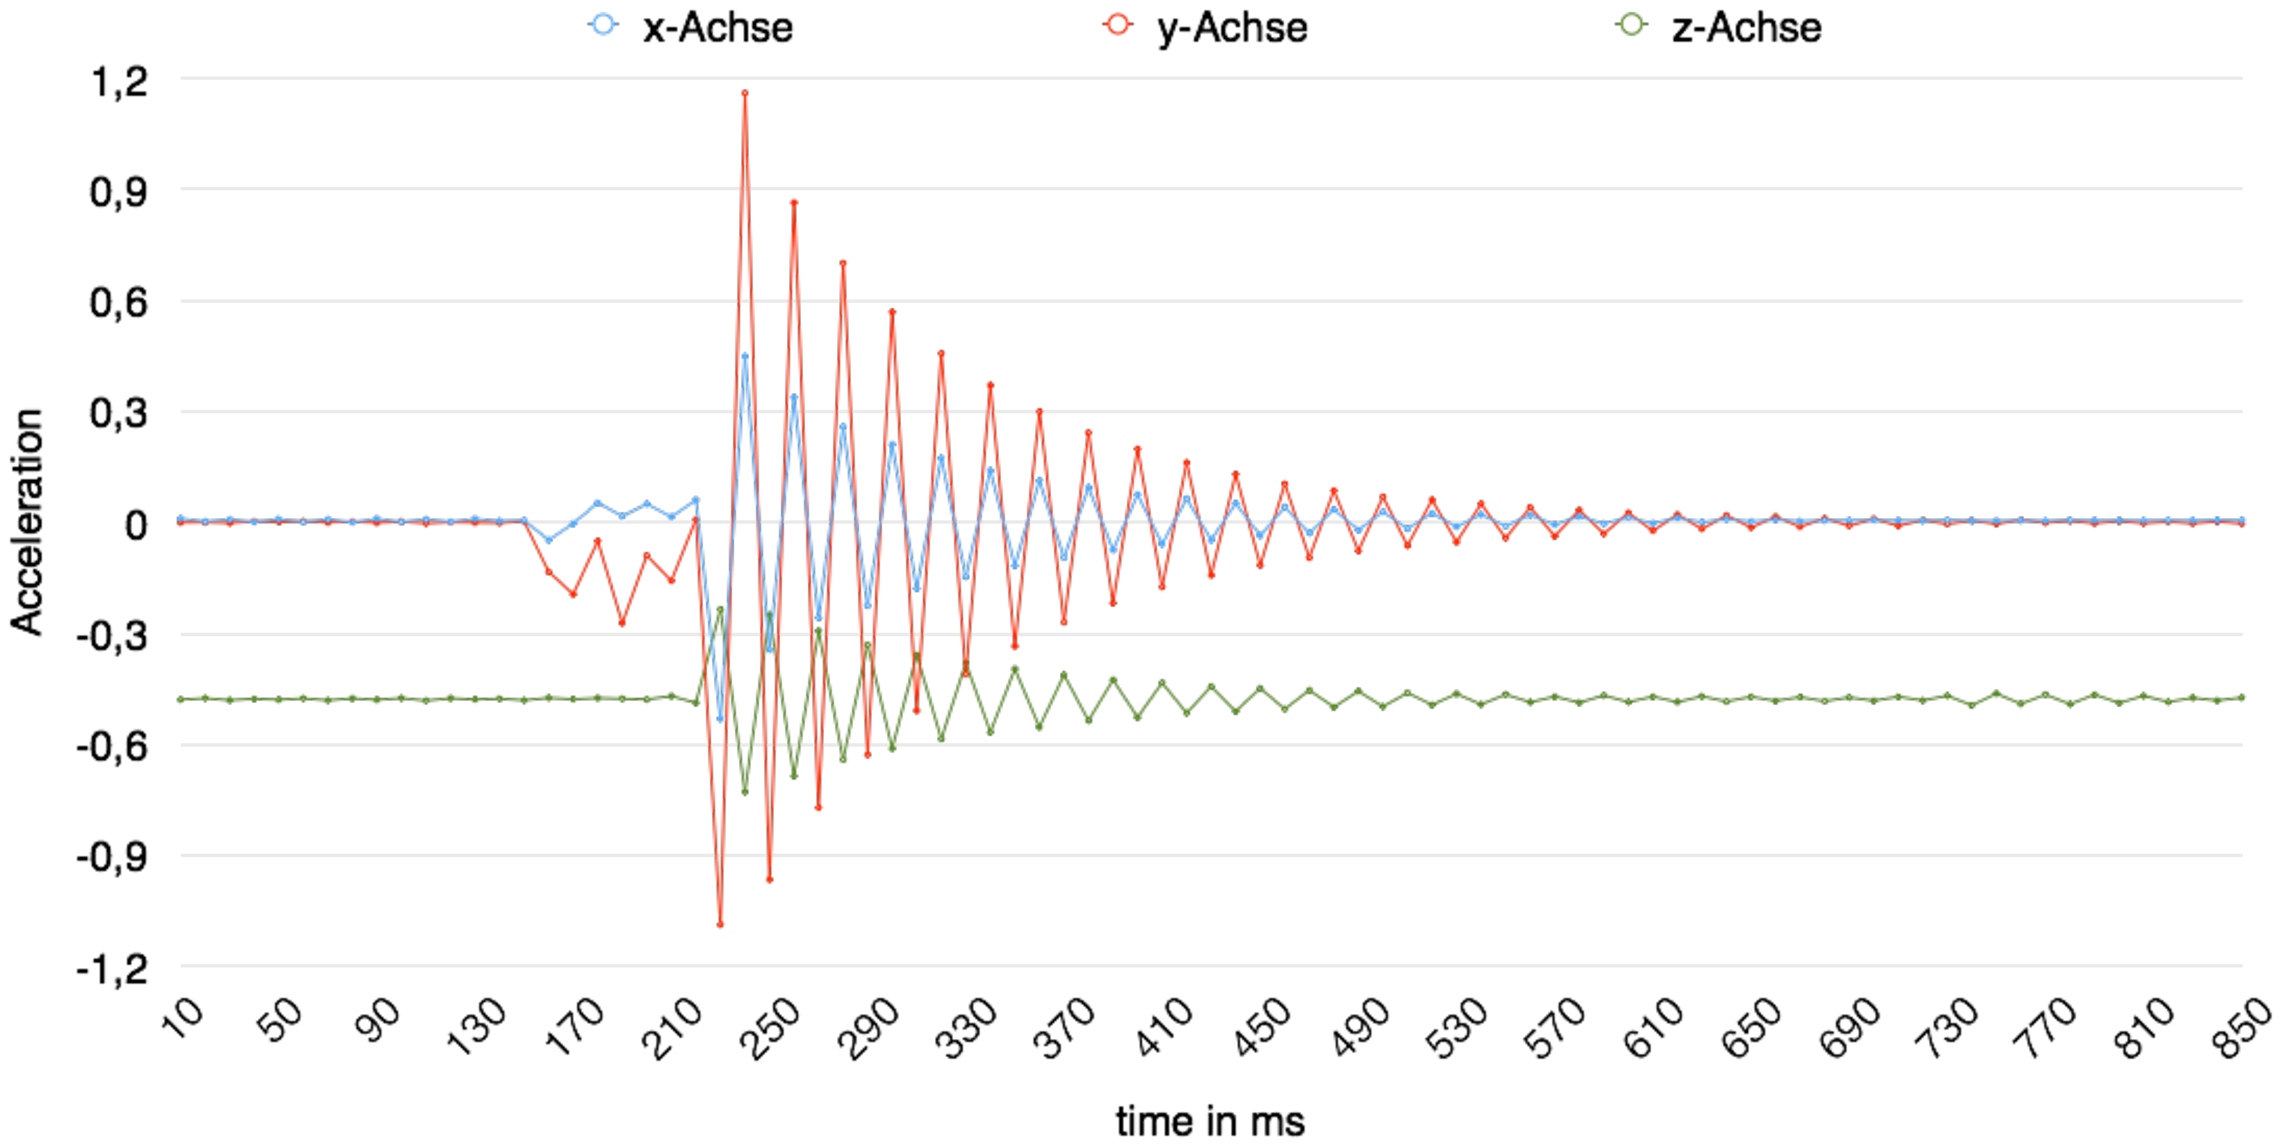
\includegraphics[width=1.0\textwidth]{kapitel4/acceleroLang.pdf}
    \caption{Bump-Muster Stirnseite an Stirnseite}
    \label{fig:stirnanstirn}
\end{figure}

\subsubsection{Längsseite an Längsseite}
Die Endgeräte werden aufrecht in den Händen der Anwender gehalten und werden an den Längsseiten zusammengestoßen.
\begin{figure}[H]
    \centering
    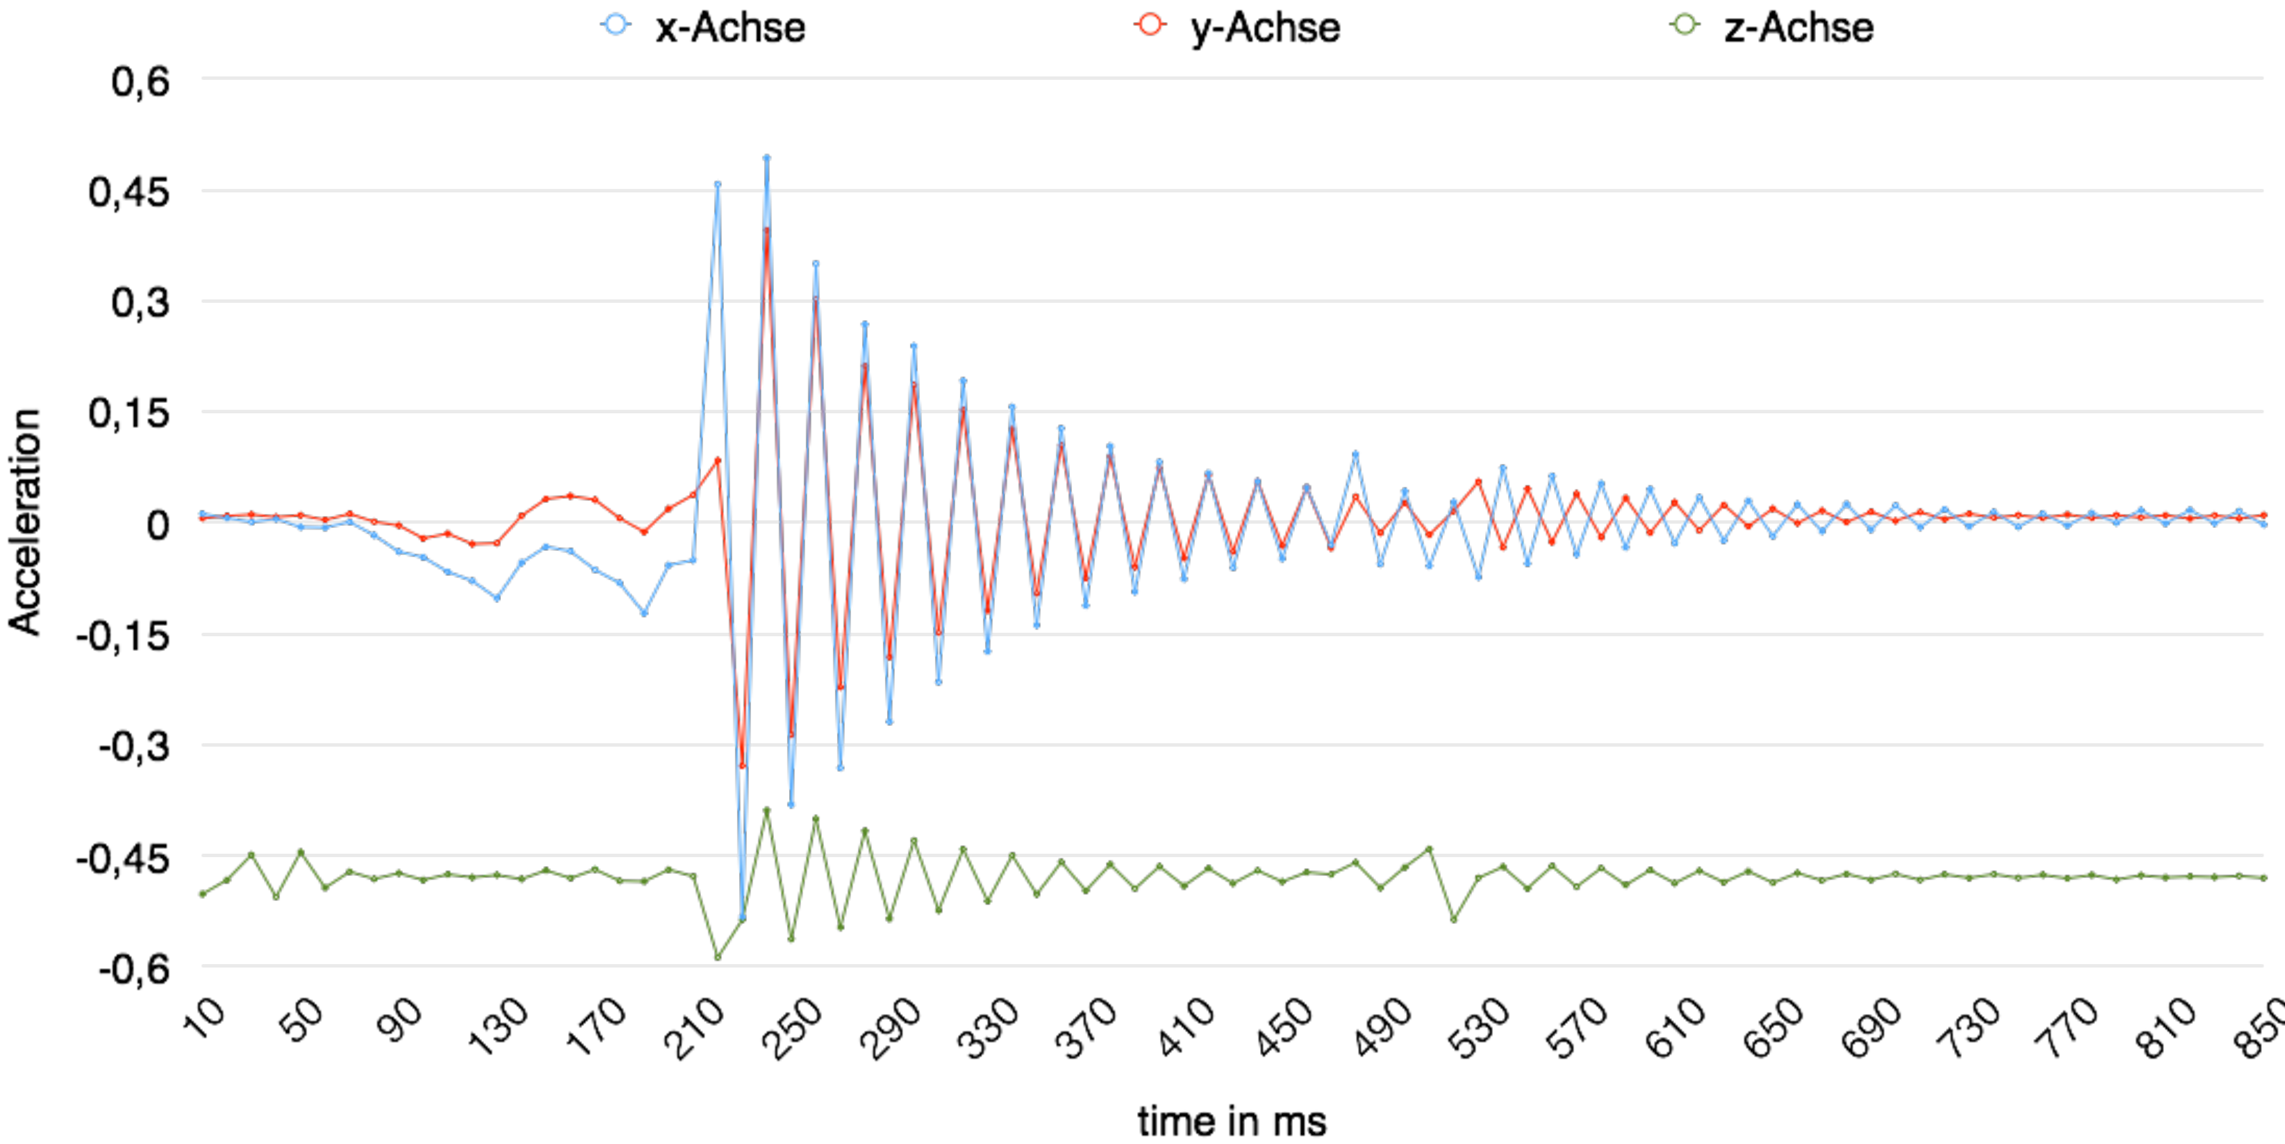
\includegraphics[width=1.0\textwidth]{kapitel4/acceleroBreit.pdf}
    \caption{Bump-Muster Längsseite an Längsseite}
    \label{fig:längsanlängs}
\end{figure}

\subsubsection{Ecke an Ecke}
Die Endgeräte werden aufrecht in den Händen der Anwender gehalten und werden an den oberen Ecken zusammengestoßen.
\begin{figure}[H]
    \centering
    \includegraphics[width=1.0\textwidth]{kapitel4/acceleroEcke.pdf}
    \caption{Bump-Muster Ecke an Ecke}
    \label{fig:eckeanecke}
\end{figure}

\subsubsection{Stirnseite aufstoßen}
Ein Endgerät wird vom Anwender aufrecht in der Hand gehalten und mit der oberen oder unteren Kante auf ein stationäres Gerät aufgestoßen.
\begin{figure}[H]
    \centering
    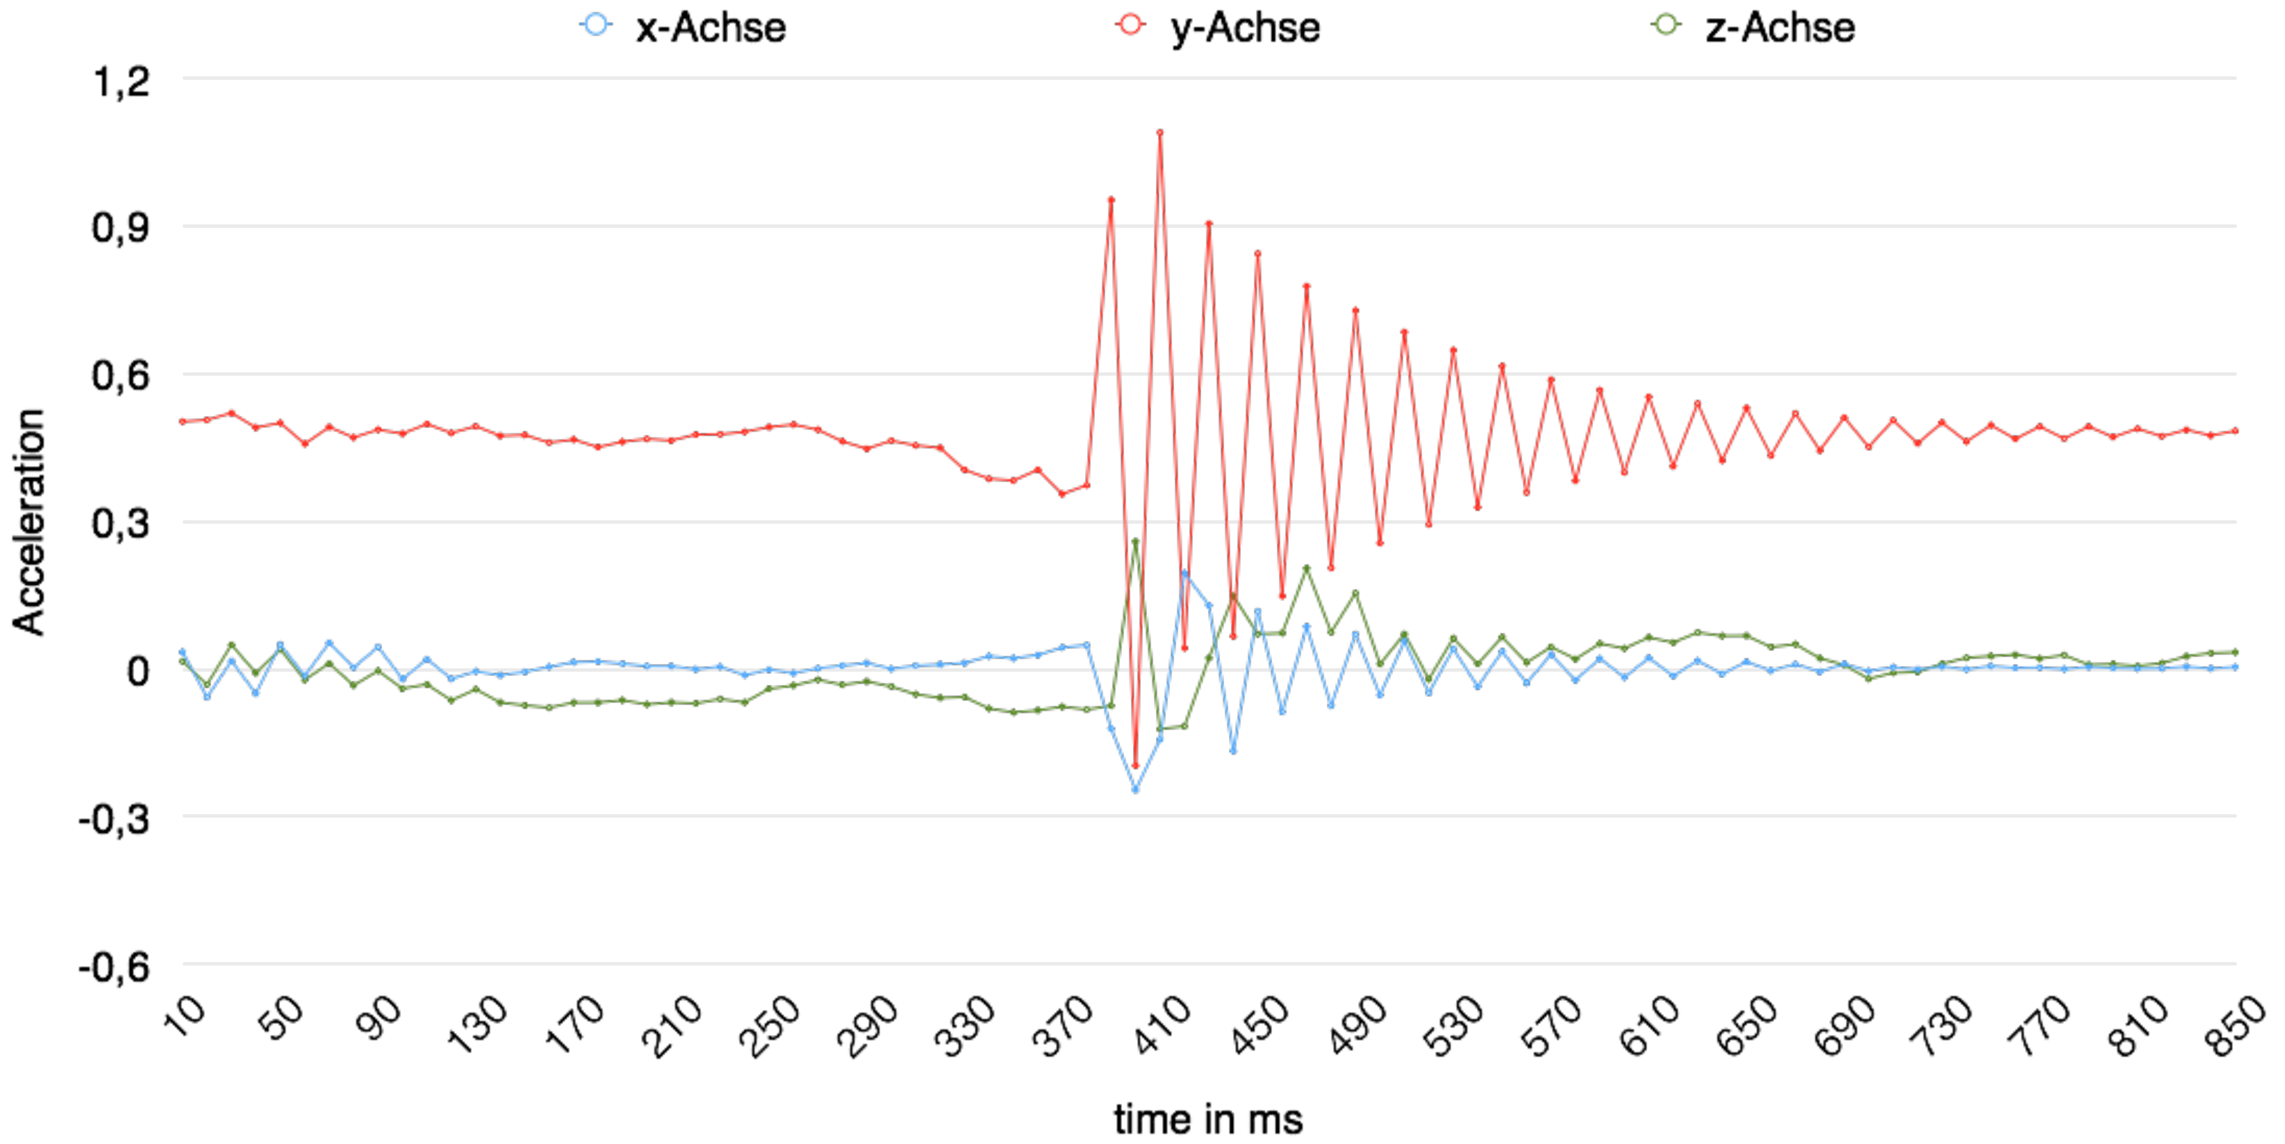
\includegraphics[width=1.0\textwidth]{kapitel4/acceleroOben.pdf}
    \caption{Bump-Muster Stirnseite aufstoßen}
    \label{fig:aufstossen}
\end{figure}

\subsubsection{Erkenntnisse aus den Versuchen}
Jede Bump-Variante generiert ein etwas anderes Muster. Es gibt jedoch Gemeinsamkeiten, die einen Bump typisieren und von anderen Bewegungen eines Benutzers unterscheiden. Die folgenden Charakteristiken können aus den Daten abgeleitet werden:
\begin{enumerate}
  \item Der Aufprall generiert initial eine hoch ausschlagende Flanke.
  \item Die nachfolgenden Daten sind alternierende Spitzen.
\end{enumerate}

\subsection{Algorithmus zur Mustererkennung}
Basierend auf den Beobachtungen aus den Versuchen, überprüft der Algorithmus die Daten des Beschleunigungssensors in zwei Schritten. Im ersten Schritt werden die Daten aller Achsen auf hoch ausschlagenden Flanken überprüft, welche einen Indikator für einen Bump darstellen. Dafür wird jeder Wert zwischengespeichert und mit dem Folgewert der Abstand (Siehe Abbildung \ref{fig:bump}) zwischen den Werten berechnet. 

\begin{figure}[H]
    \centering
    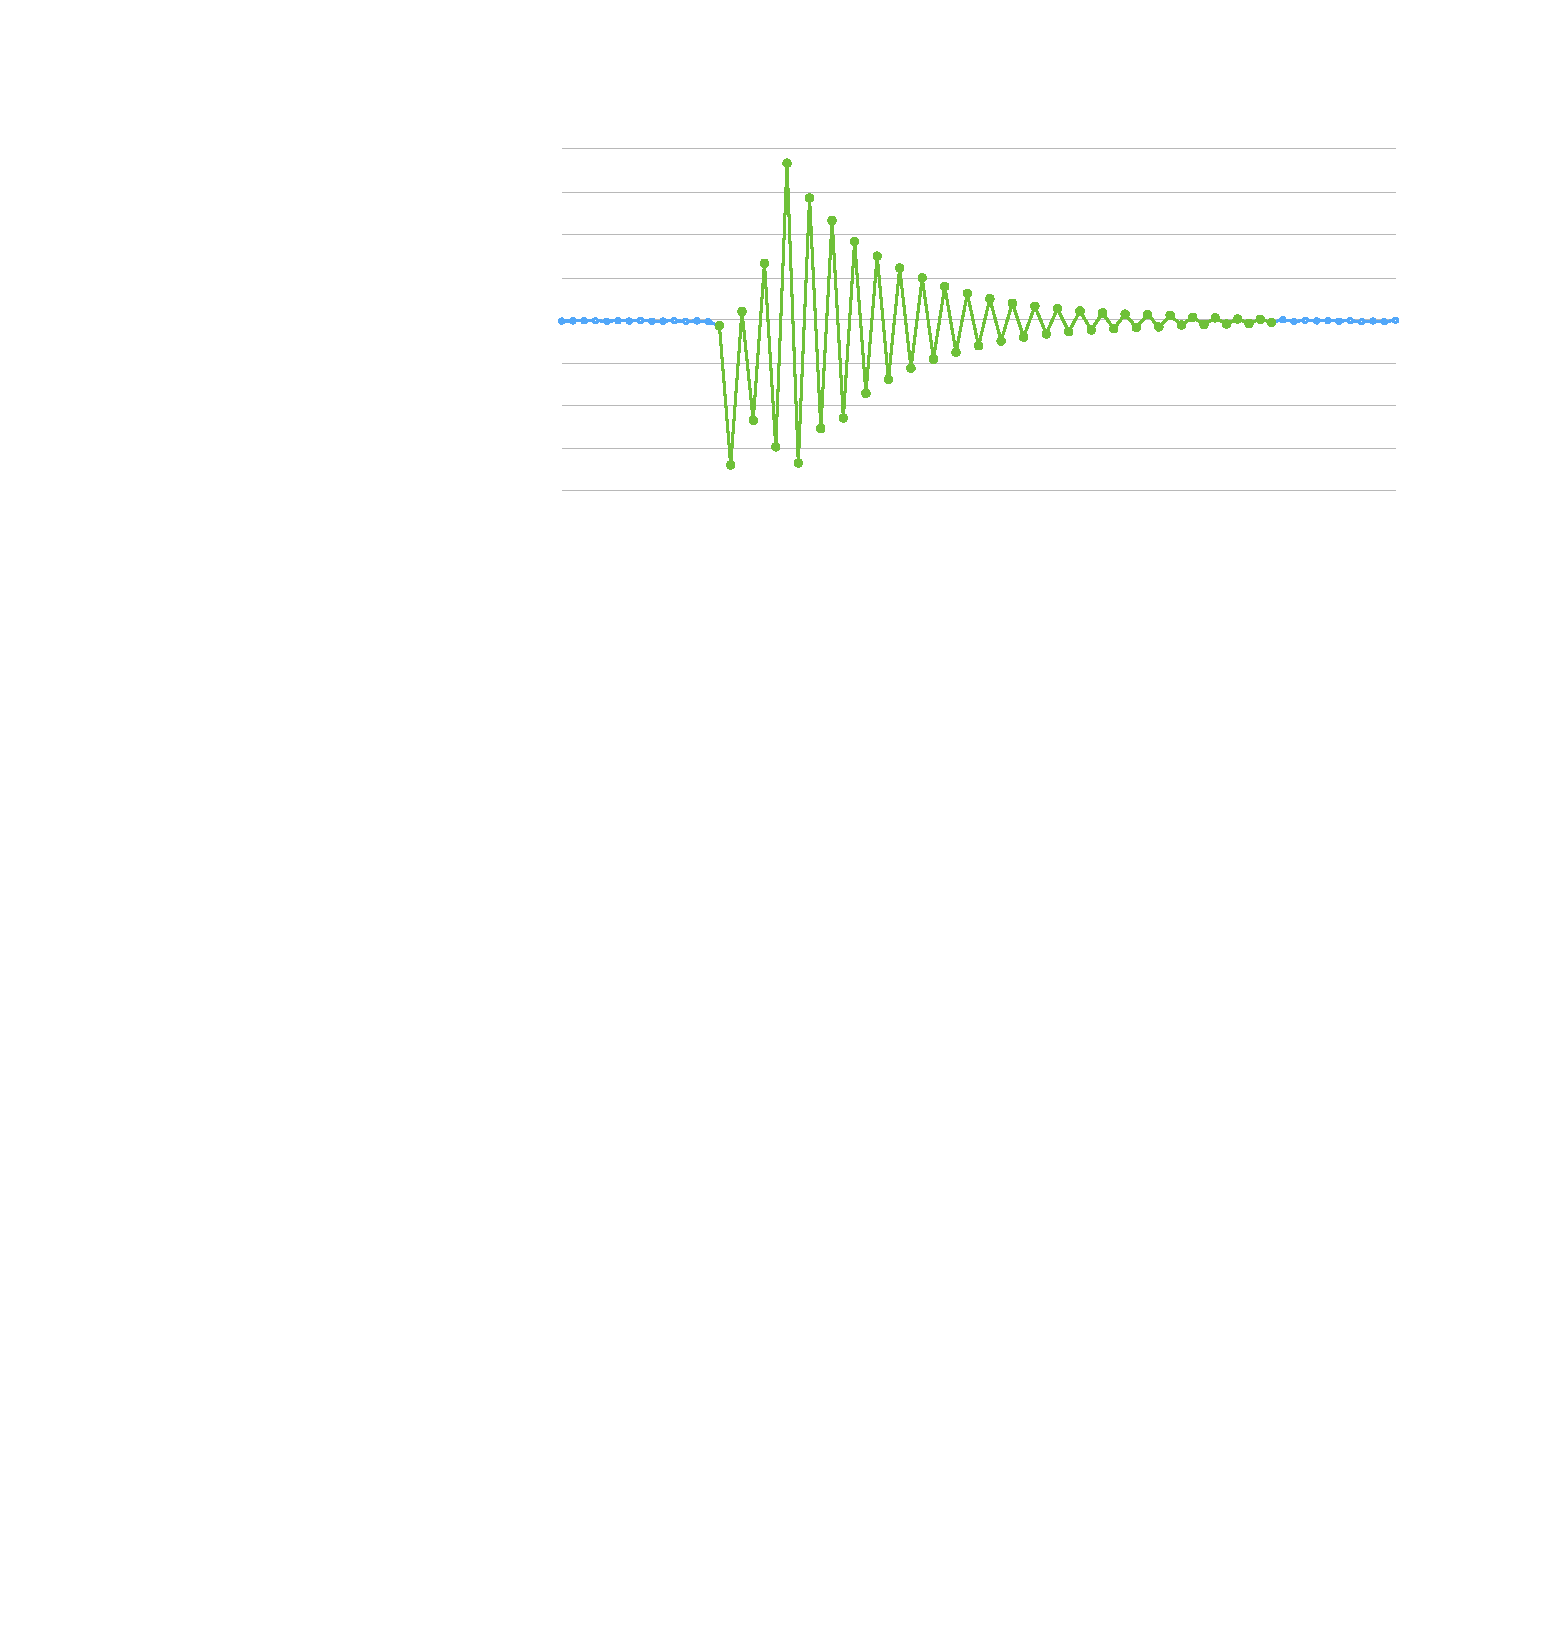
\includegraphics[width=1.0\textwidth]{kapitel4/acceleroBump.pdf}
    \caption{Algorithmische Erkennung eines Bumps}
    \label{fig:bump}
\end{figure}

Hat der Algorithmus initiale Flanken erkannt, wird im nächsten Schritt die durch die Kraft des Bumps beeinflussten Daten in einem Vektor für jede Achse aufgezeichnet. Um zu verifizieren, dass ein Bump stattgefunden hat, läuft anschließend eine Schleife über die Vektoren und zählt die Spitzen. Sind nur Spitzen im Vektor vorhanden, handelt es sich um einen Bump.

\newpage
\section{Konzepte zur Identifizierung von Bump-Partnern}
\label{sec:Ident}
Um Daten zwischen Bump-Partnergeräten, in einem lokalen Netzwerk oder über einen Server, auszutauschen müssen die Endgeräte, aus allen Teilnehmern eines Netzwerkes bzw. allen Clients die mit einem Server verbunden sind, ihren jeweiligen Partner identifizieren. Folgend werden zwei Verfahren vorgestellt mit denen diese Identifizierung erfolgen kann.

\subsection{Identifizierung über iBeacon Geräte-IDs}
Über die Major- und Minor-Werte kann mit iBeacon jedem Endgerät eine einzigartige ID zugeordnet werden mit der Endgeräte identifiziert werden können. Um diese ID zwischen Bump-Partnern auszutauschen, wird auf beiden Geräten iBeacon zum Zeitpunk des Bumps für kurze Zeit aktiviert. Gerade lange genug, damit die Endgeräte alle aktiven Beacons in ihrem Umfeld sehen können. Dadurch besitzt jedes Gerät eine Liste an Beacons die zu einen bestimmten Zeitpunkt an einem Bump, in ihrer Empfangsreichweite, beteiligt waren. Können die Endgeräte jeweils nur ein anderes Beacon sehen, haben Sie ihren Bump-Partner identifiziert. Ist mehr als ein Beacon sichtbar, fanden mehrere Bumps zeitgleich statt. In diesen Fällen können die Partner, über die Entfernung der Geräte zueinander, ermittelt werden. Bei den Geräten mit dem geringsten Abstand handelt es sich um die Bump-Partner. Die Erkennung der Partnergeräte über die Entfernung macht es erforderlich, dass zeitgleiche Bumps mindestens einige Zentimeter voneinander entfernt stattfinden. Dies stellt sicher, dass eine falsche Zuordnung durch ungenaue Abstandsmessungen vermieden wird.

\subsection{Identifizierung durch charakteristische Bump-Daten}
Ein Bump ist ein Ereignis, bei dem beteiligte Geräte verschiedene Daten erfassen können, die jeden Bump einzigartig charakterisieren. Eine Kombination aus Zeitpunkt und Standort bietet in den meisten Fällen eine ausreichende Datenbasis, um Bumps voneinander unterscheiden zu können. Der Zeitpunkt des Bumps kann mit einem Timestamp festgehalten werden. Bei der Nutzung von Timestamps muss jedoch beachtet werden, dass die Uhren der Geräte nicht synchron laufen. Um möglichst übereinstimmende Timestamps zu erhalten, sollte die Applikation deshalb die Systemuhr in bestimmten Zeitintervallen synchronisieren. Die Position der Endgeräte zum Zeitpunkt des Bumps kann über \ac{GPS} Koordinaten erfasst werden. Da sich Geräte bei einem Bump berühren, sollten im besten Falle die Koordinaten, die auf beiden Geräte ermittelt werden, übereinstimmen. Bei der Nutzung von \ac{GPS}muss aber beachtet werden, dass nicht immer eine genaue Positionsbestimmung garantiert ist. Trotz der etwaigen Abweichungen von sowohl Timestamp als auch \ac{GPS}, sollte eine Kombination dieser Daten in den meisten Fällen ausreichen, um Endgeräte zuverlässig einem Bump zuordnen zu können.

\subsection{Vergleich der Konzepte}
Der Vergleich von Timestamps und \acs{GPS}-Positionsdaten sollte in den meisten Fällen zuverlässige Zuordnung von Bump-Partnern ermöglichen. Jedoch erreicht das System seine Grenzen, wenn mehrere Bumps zum selben Zeitpunkt und am selben Standort stattfinden. Die potenzielle Ungenauigkeit von \ac{GPS} kann dazu führen, dass die jeweiligen Partnergeräte nicht zugeordnet werden können. Des weiteren kann gerade im Inneren von Gebäuden dieses System unter Umständen durch den verminderten Satellitenempfang gar nicht oder nur mit Einschränkungen genutzt werden. Zum Vergleich ist das System mit iBeacon und GeräteIDs in Innenräumen besser nutzbar als \ac{GPS} und ermöglicht, den Abstand zwischen Endgeräten genauer zu bestimmen. Die Identifizierung durch die Entfernungsmessung mit iBeacon besitzt aber auch ihre Grenzen. Finden zeitgleich Bumps in nur wenigen Zentimetern Entfernung zueinander statt, ist auch hier keine fehlerfreie Zuordnung garantiert. Im Vergleich ist iBeacon genauer als \acs{GPS} und sollte in den Fällen in denen der Abstand der Geräte entscheidend ist die besseren Ergebnisse erzielen.

\newpage
\section{Konzepte zum Datenaustausch}
\label{sec:Austausch}
Der Datenaustausch zwischen Endgeräten lässt sich über zwei verschiedene Ansätze realisieren. Zum einen können Daten direkt zwischen den Geräten über ein lokales Netzwerk getauscht werden und zum anderen über einen zentralen Server. Für beide Varianten werden folgend Konzepte vorgestellt, in denen sich Endgeräte identifizieren und Daten austauschen können.

\subsection{Datenaustausch über lokale Netzwerke}
Mit Hilfe von drahtlosen Netzwerktechnologien kann Datenaustausch zwischen Endgeräten entweder über ein WLAN-Infrastrukturnetzwerk oder durch die Bildung eines Ad-Hoc Netzwerkes realisiert werden. Unabhängig von der Topologie des Netzwerkes läuft die Kommunikation zwischen den Netzwerkteilnehmern über Netzwerkdienste. Entscheidend ist dabei, dass sich die an einem Bump-Event beteiligten Geräte im Computernetzwerk gegenseitig identifizieren können. Folgend wird einleitend beschrieben wie die beiden in \ref{sec:Ident} beschriebenen Konzepte in lokalen Netzwerken angewendet werden. Anschließend werden für beide Möglichkeiten der genaue Ablauf des Verbindungsaufbaus zwischen den Geräten beschrieben.

\subsubsection{Geräteidentifizierung in lokalen Netzwerken}
Es werden zwei Maßnahmen ergriffen, mit denen sichergestellt werden soll, dass sich die an einem Bump beteiligten Geräte zuverlässig identifizieren. Im ersten Schritt wird dazu die Anzahl an Netzwerkteilnehmern, die den selben Netzwerkdienst zeitgleich verwenden, verringert. Dazu wird der Netzwerkdienst, der von der Bump-Applikation angeboten wird, erst gestartet, nachdem das Bump-Event stattgefunden hat und wieder gestoppt, sobald zwischen den Bump-Partnern eine Verbindung aufgebaut wurde. Dadurch ist der Netzwerkdienst nur für kurze Zeit bei jenen Endgeräten aktiv, die zum gleichen Zeitpunkt einen Bump durchgeführt haben. Der Zeitraum, in dem der Netzwerkdienst von den Bump-Partner angeboten und gesucht wird, ist sehr kurz, in den meisten Fällen werden deswegen immer nur Bump-Partner gleichzeitig den selben Netzwerkdienst nutzen, wodurch eine weitere Identifizierung gar nicht nötig wäre (Siehe Abbildung \ref{fig:dienste} a).

\begin{figure}[H]
    \centering
    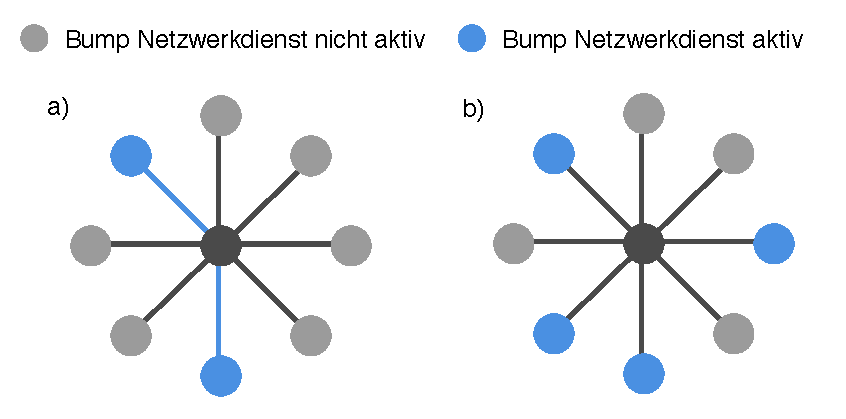
\includegraphics[width=\linewidth]{kapitel4/netzwerkdienste.pdf}
    \caption{Netzwerkdienste in einem Infrasturkturnetzwerk}
    \label{fig:dienste}
\end{figure}

Da jedoch nicht sichergestellt werden kann, dass in der Zeitspanne in der Bump-Partner den Netzwerkdienst nutzen, kein weiterer Bump auftritt und dadurch mehr als zwei Engeräte den Netzwerkdienst nutzen (Siehe Abbildung \ref{fig:dienste} b), wird zusätzlich noch eine der in Abschnitt \ref{sec:Ident} beschriebenen Methode benötigt, mit der sich Bump-Partner im Netzwerk identifizieren können (Siehe Abbildung \ref{fig:diensteIdent}).

\begin{figure}[H]
    \centering
    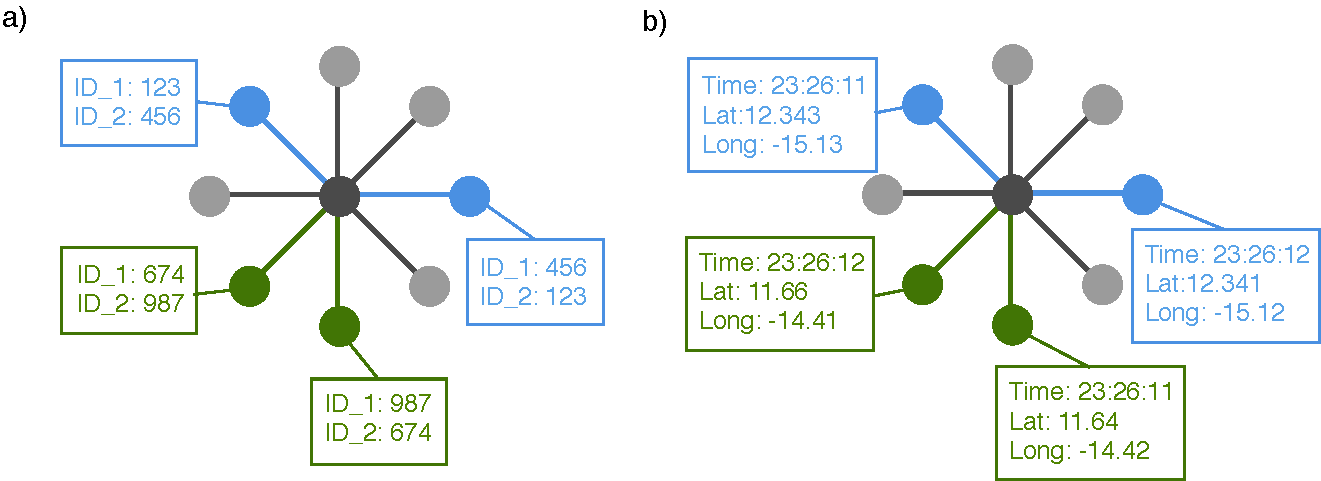
\includegraphics[width=\linewidth]{kapitel4/netzwerkdiensteIdent.pdf}
    \caption{Identifizierung von Netzwerkteilnehmern}
    \label{fig:diensteIdent}
\end{figure}

\newpage
\subsubsection{Ablauf mit iBeacon Geräte-IDs}
Wird auf einem Gerät ein Bump registriert, ist der erste Schritt die Generierung von Zufallszahlen für den Major- und Minor-Wert von iBeacon. Diese Zahlen bilden eine eindeutige ID, mit der sich jedes Gerät im Netzwerk identifizieren kann. Anschließend wird iBeacon aktiviert, die Geräte können sich gegenseitig sehen, GeräteIDs lesen und die Distanz zu allen sichtbaren Beacons erfassen. Ist mehr als ein Beacon sichtbar, wird jenes ermittelt, welches die geringste Distanz zum suchenden Gerät aufweist. Die GeräteID dieses Geräts wird lokal gespeichert und iBeacon wird deaktiviert. Anschließend startet die DiscoveryPhase des Multipeer-Connectivity-Frameworks. In dieser Phase agiert das Gerät, dessen Minor Wert den kleineren Zahlenwert aufweist, als Advertiser und bietet einen Netzwerkdienst an. Die discoveryInfo dieses Dienstes enthält die durch Major und Minor gebildete GeräteID des Advertisers. Das Gerät mit dem höheren Zahlenwert ist der Browser und sucht den Dienst des Advertisers. Diese Aufgabenverteilung verhindert, dass Probleme beim Verbindungsaufbau auftreten, sollten sich die Geräte gleichzeitig zu einer Session einladen.
Findet der Browser diesen Dienst, kann er die GeräteID des Advertisers mit der GeräteID vergleichen, die das zu Beginn ermittelte Beacon aufweist. Stimmen die IDs überein, handelt es sich bei dem Advertiser um den Bump-Partner und der Browser kann eine Session erstellen und eine Einladung zu dieser an den Advertiser schicken. Mit dieser Einladung wird in der contextData wiederum die GeräteID des Browsers mitgeschickt. Damit kann der Advertiser überprüfen, ob er auch wirklich von seinem Partner eingeladen wird und nicht von jemand anderem. Haben die Geräte eine Verbindung aufgebaut, können Sie über die Methoden des Frameworks die gewünschten Daten austauschen, und anschließend die Session verlassen. 

Der beschriebene Ablauf kann auch noch einmal im folgenden UML Diagramm nachvollzogen werden.

\begin{figure}[H]
    \centering
    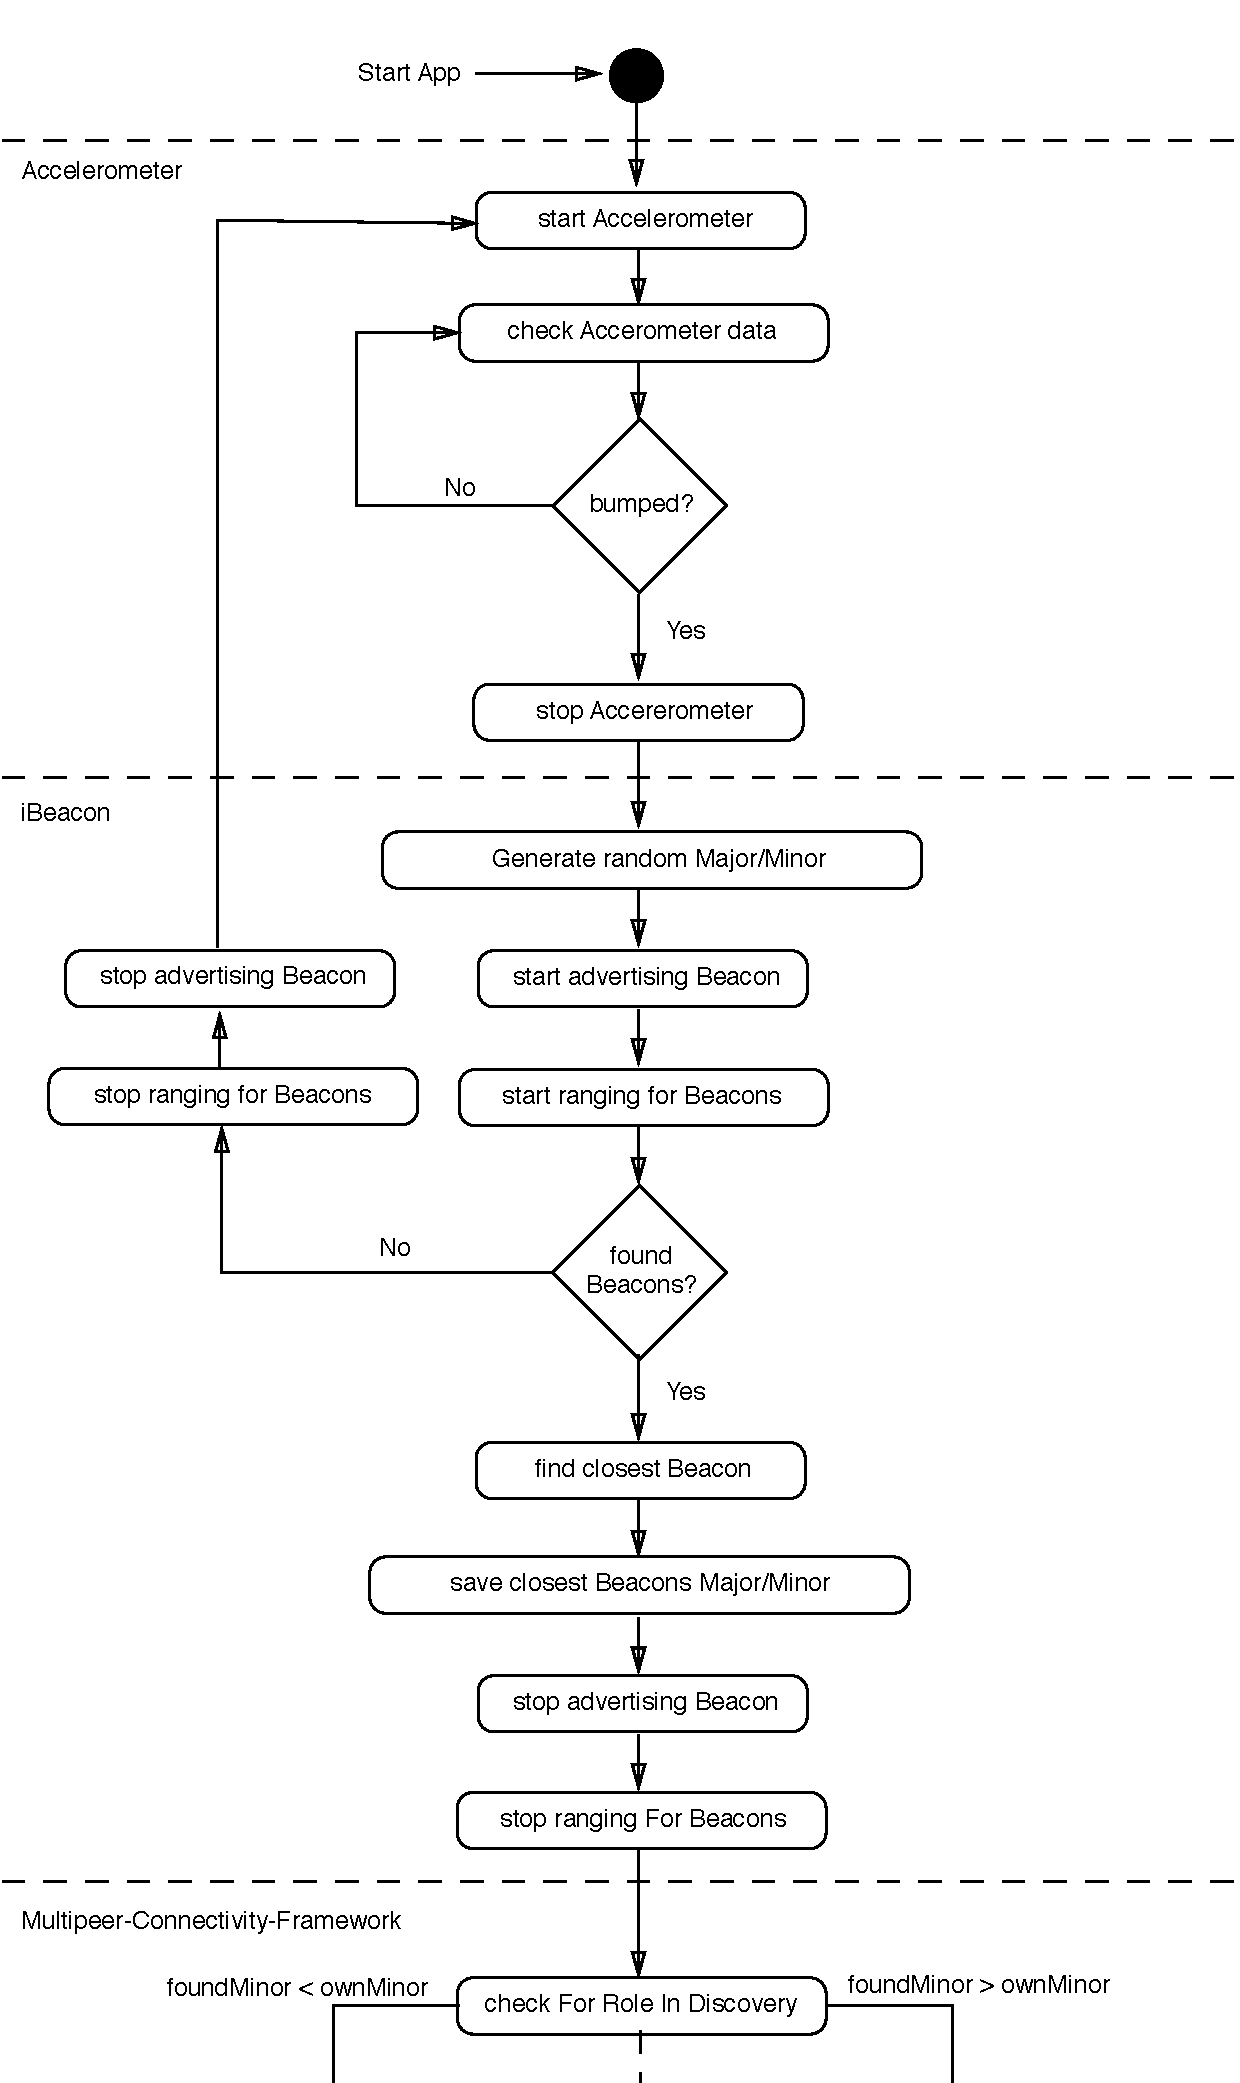
\includegraphics[width=\linewidth]{kapitel4/umlkurz1.pdf}
    \label{umlBecon1}
    \caption{System mit iBeacon UML Diagramm}
\end{figure}
\begin{figure}[H]
    \centering
    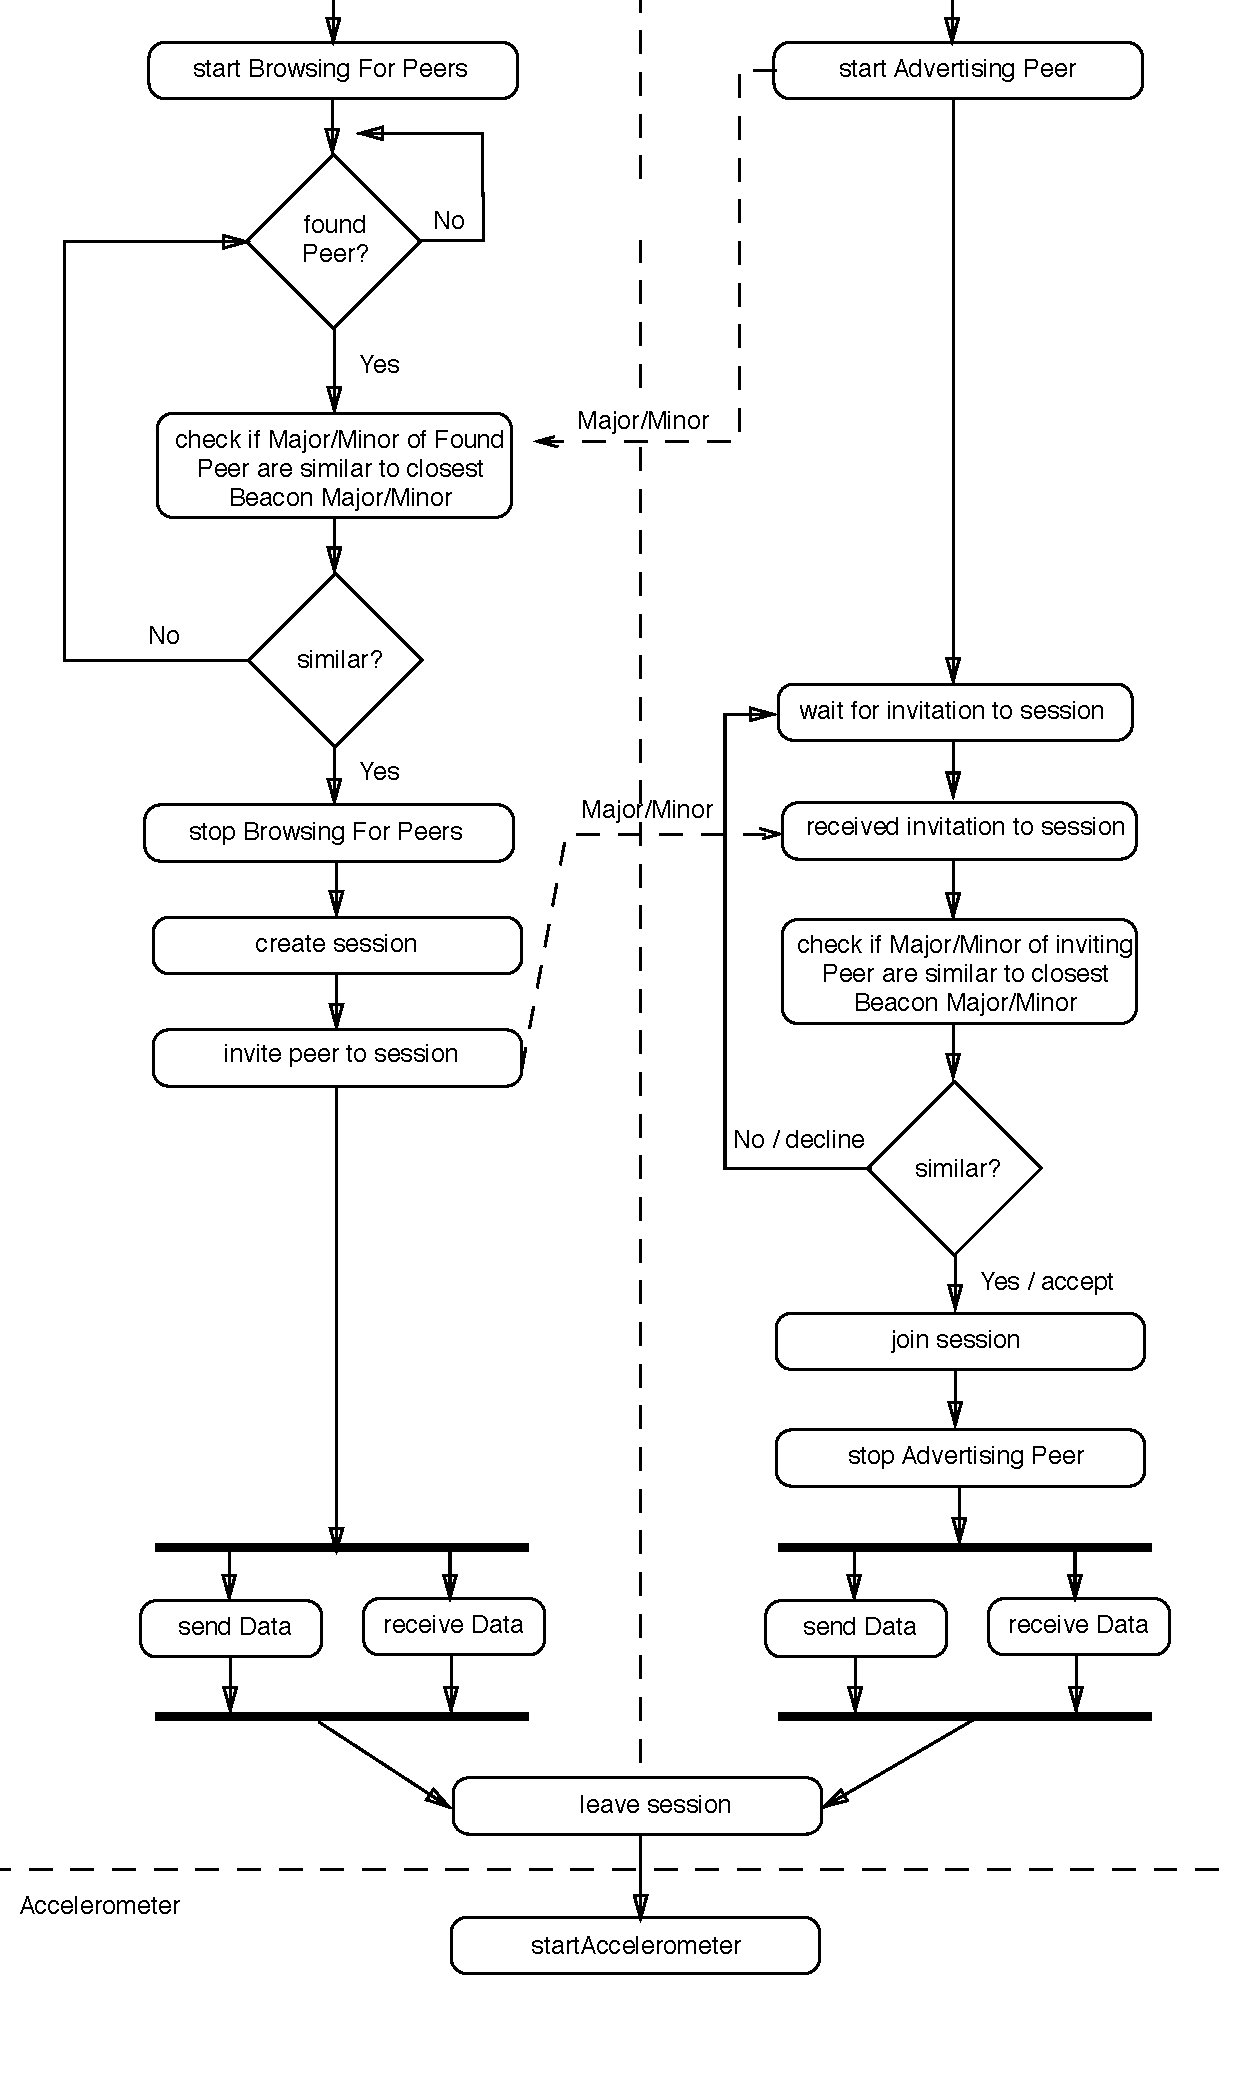
\includegraphics[width=\linewidth]{kapitel4/umlkurz2.pdf}
    \label{umlBecon2}
    \caption{System mit iBeacon UML Diagramm}
\end{figure}

\subsubsection{Ablauf mit Timestamp und GPS}
Mit Timestamp und \ac{GPS} läuft der Verbindungsaufbau etwas anders ab, als mit iBeacon. Zuerst werden die \ac{GPS} Daten der Endgeräte erfasst und lokal gespeichert. Im nächsten Schritt eröffnen beide Endgeräte einen Browser- und Advertiser-Dienst mit einem gemeinsamen Bezeichner. Die zuvor gespeicherten \ac{GPS} Daten werden bei beiden Geräten in der discoveryInfo zusammen mit einer generierten Zufallszahl untergebracht. Beide Geräte können nun auf Timestamp und \ac{GPS} Daten der gefundenen Geräte zugreifen und Timestamp und \ac{GPS} Daten mit den eigenen abgleichen. Stimmen die gefundenen Daten mit den eigenen überein, wurde identifiziert welches Gerät zu einer Session eingeladen werden muss. Wer diese Session erstellt und den Partner zu dieser einlädt, wird über die generierte Zufallszahl die ebenfalls in der discoveryInfo gespeichert wird, ausgehandelt. Nachdem die Session zustande gekommen ist, werden die Netzwerkdienste deaktiviert und der Datenaustausch kann erfolgen.

Der beschriebene Ablauf ist im folgenden UML Diagramm noch einmal dargestellt.

\begin{figure}[H]
    \centering
    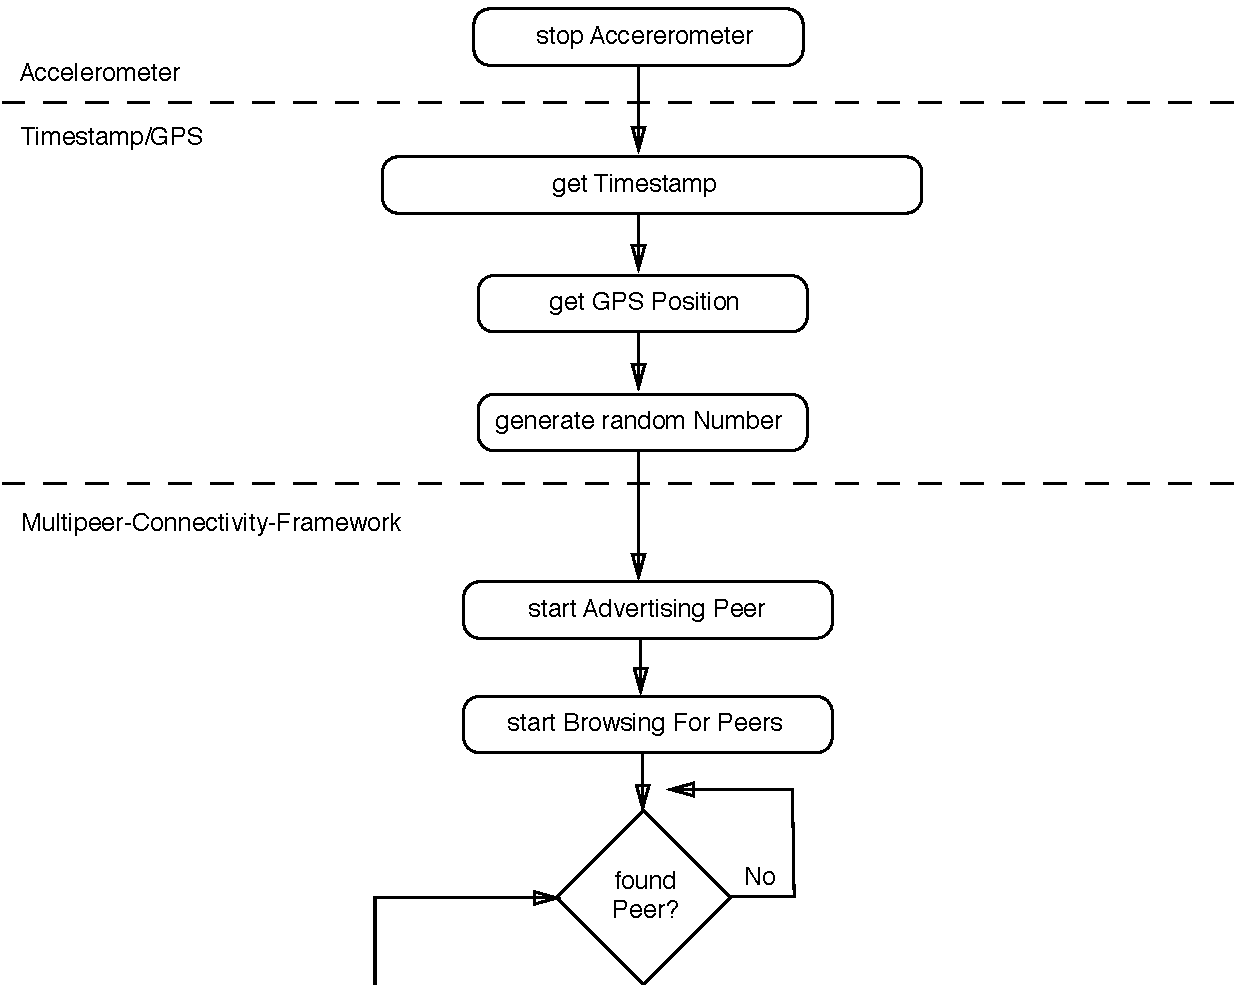
\includegraphics[width=\linewidth]{kapitel4/umlGPS.pdf}
    \label{umlGPS1}
    \caption{System mit Timestamp und GPS UML Diagramm}
\end{figure}
\begin{figure}[H]
    \centering
    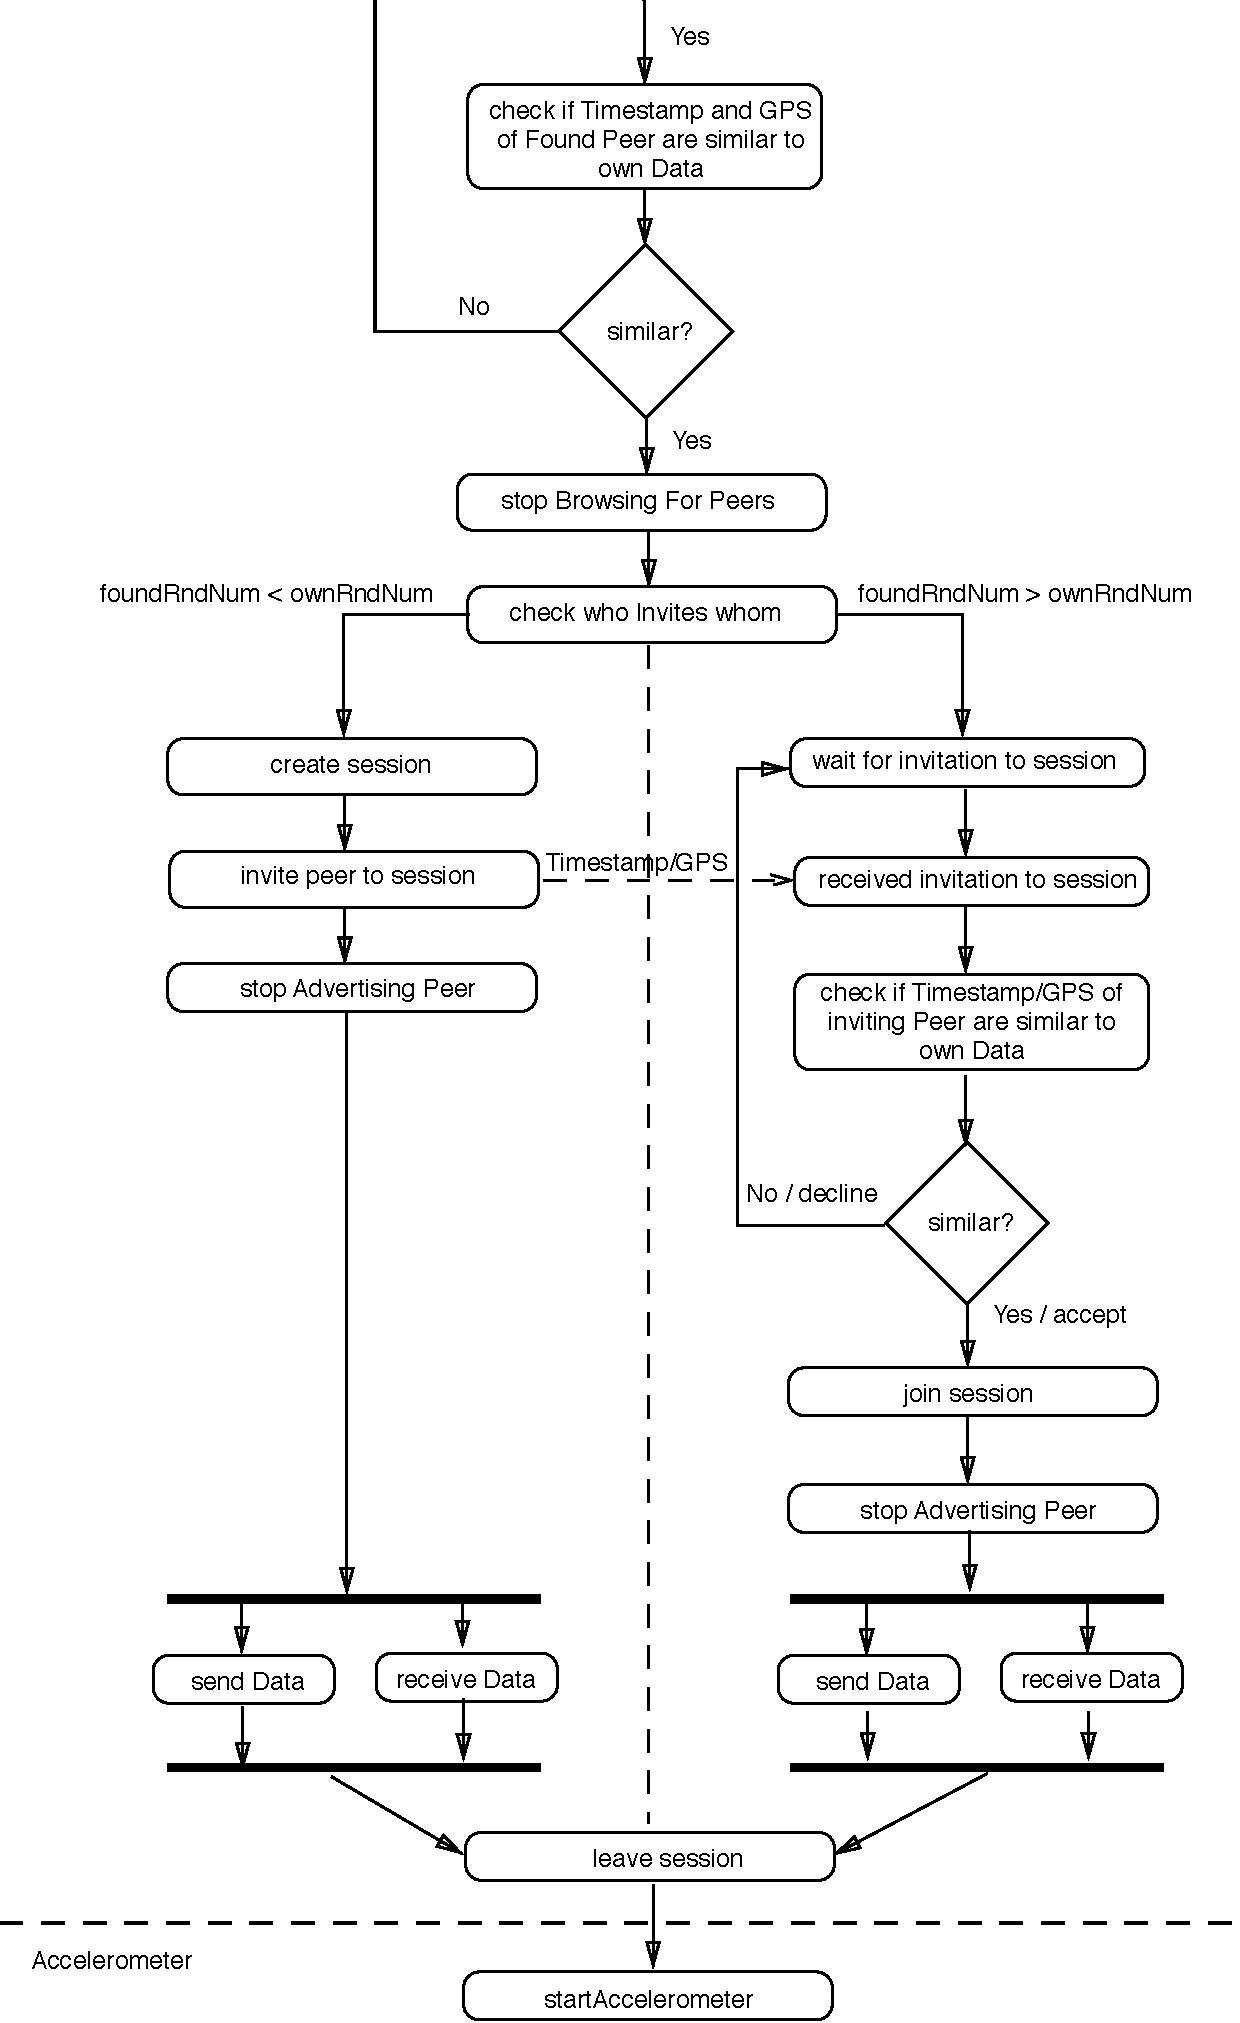
\includegraphics[width=\linewidth]{kapitel4/umlGPS2.pdf}
    \label{umlGPS2}
    \caption{System mit Timestamp und GPS UML Diagramm}
\end{figure}

\subsection{Datenaustausch über Webserver}
\label{sec:AustauschWebserver}

Die Kommunikation der Endgeräte über Webserver ist eine alternative Möglichkeit den Datenaustausch zwischen den Endgeräten zu implementieren. Im folgend beschriebenen System werden zwei Server genutzt, die nach verschiedenen Aufgaben aufgeteilt sind. Einer der Server, im folgenden als Fileserver bezeichnet, dient als Austausch Plattform für die von den Anwendern ausgewählten Daten. Diese werden von den Endgeräten auf den Server hochgeladen und sind dort anschließend unter einer bestimmten \acs{URL} erreichbar. Für die Übermittlung der \acs{URL} von Sender zu Empfänger ist der zweite Server, im folgenden als Messaging-Server bezeichnet, zuständig. Mit diesem Server verbinden sich die Bump-Partner über WebSockets und sind damit Teil eines Nachrichtensystems, mit dem der Server Nachrichten von allen verbundenen Endgeräten empfangen, aber auch senden kann. Damit der Matchmaking-Server die Nachrichten an die richtigen Geräte weiterleiten kann, müssen diese wie auch in lokalen Netzwerken identifiziert werden. Wie die Kommunikation mit den einzelnen Servern genau abläuft, wird folgend erklärt.

\subsubsection{Ablauf der Kommunikation}
Verbinden sich Clients über WebSockets mit einem Server, wird jeder Socket mit einer eigenen SocketId erstellt. Über diese SocketID kann der Server einem bestimmten Client gezielt Nachrichten zuschicken. Da die Bump-Partnergeräte die SocketID des anderen nicht kennen, muss die SocketID auf dem Server mit zusätzlichen Informationen verknüpft werden, durch die der Server Bump-Partner einander zuordnen kann. Aus diesem Grund senden die Clients beim verbinden zum Server ihre GeräteIDs oder Timestamp und \acs{GPS} an den Server. Dieser erstellt anschließend ein User Objekt, speichert in diesem die SocketID zusammen mit den Identifikationsinformationen und fügt es einer Liste mit allen verbundenen Clients hinzu. Möchten Endgeräte ihren Partnern eine Nachricht schicken, müssen sie z.B. nur die GeräteID ihrer Partners mitsenden und der Server kann anhand dieser ID die SocketID über das User Objekt ermitteln und die Nachricht weiterleiten. Sobald sich beide Partnergeräte verbunden haben, informiert der Server die jeweiligen Clients darüber. Daraufhin können die Endgeräte die vom Anwender ausgewählten Daten auf den Fileserver hochladen, der ihnen, sobald der upload abgeschlossen ist, eine \acs{URL} zurückliefert, an der die Daten gespeichert sind. Diese \acs{URL} kann anschließend über den Messaging-Server an das Partnergerät übermittelt werden, das darauf den Download vom Fileserver starten kann. Sobald die Endgeräte jeweils ihre Downloads abgeschlossen haben, können Sie sich vom Messaging-Server abmelden und der Datenaustausch ist abgeschlossen. Im folgenden ist ein kleiner Codeausschnitt zu finden, in dem exemplarisch einige Funktionen zur WebSocket Kommunikation für den beschriebenen Ablauf dargestellt sind. Außerdem kann der beschriebene Ablauf noch einmal im Sequenzdiagramm (\ref{fig:sequenz}) nachvollzogen werden.

\lstinputlisting[firstline=1,language=Java]{\srcloc/source.java}

\begin{figure}[H]
    \centering
    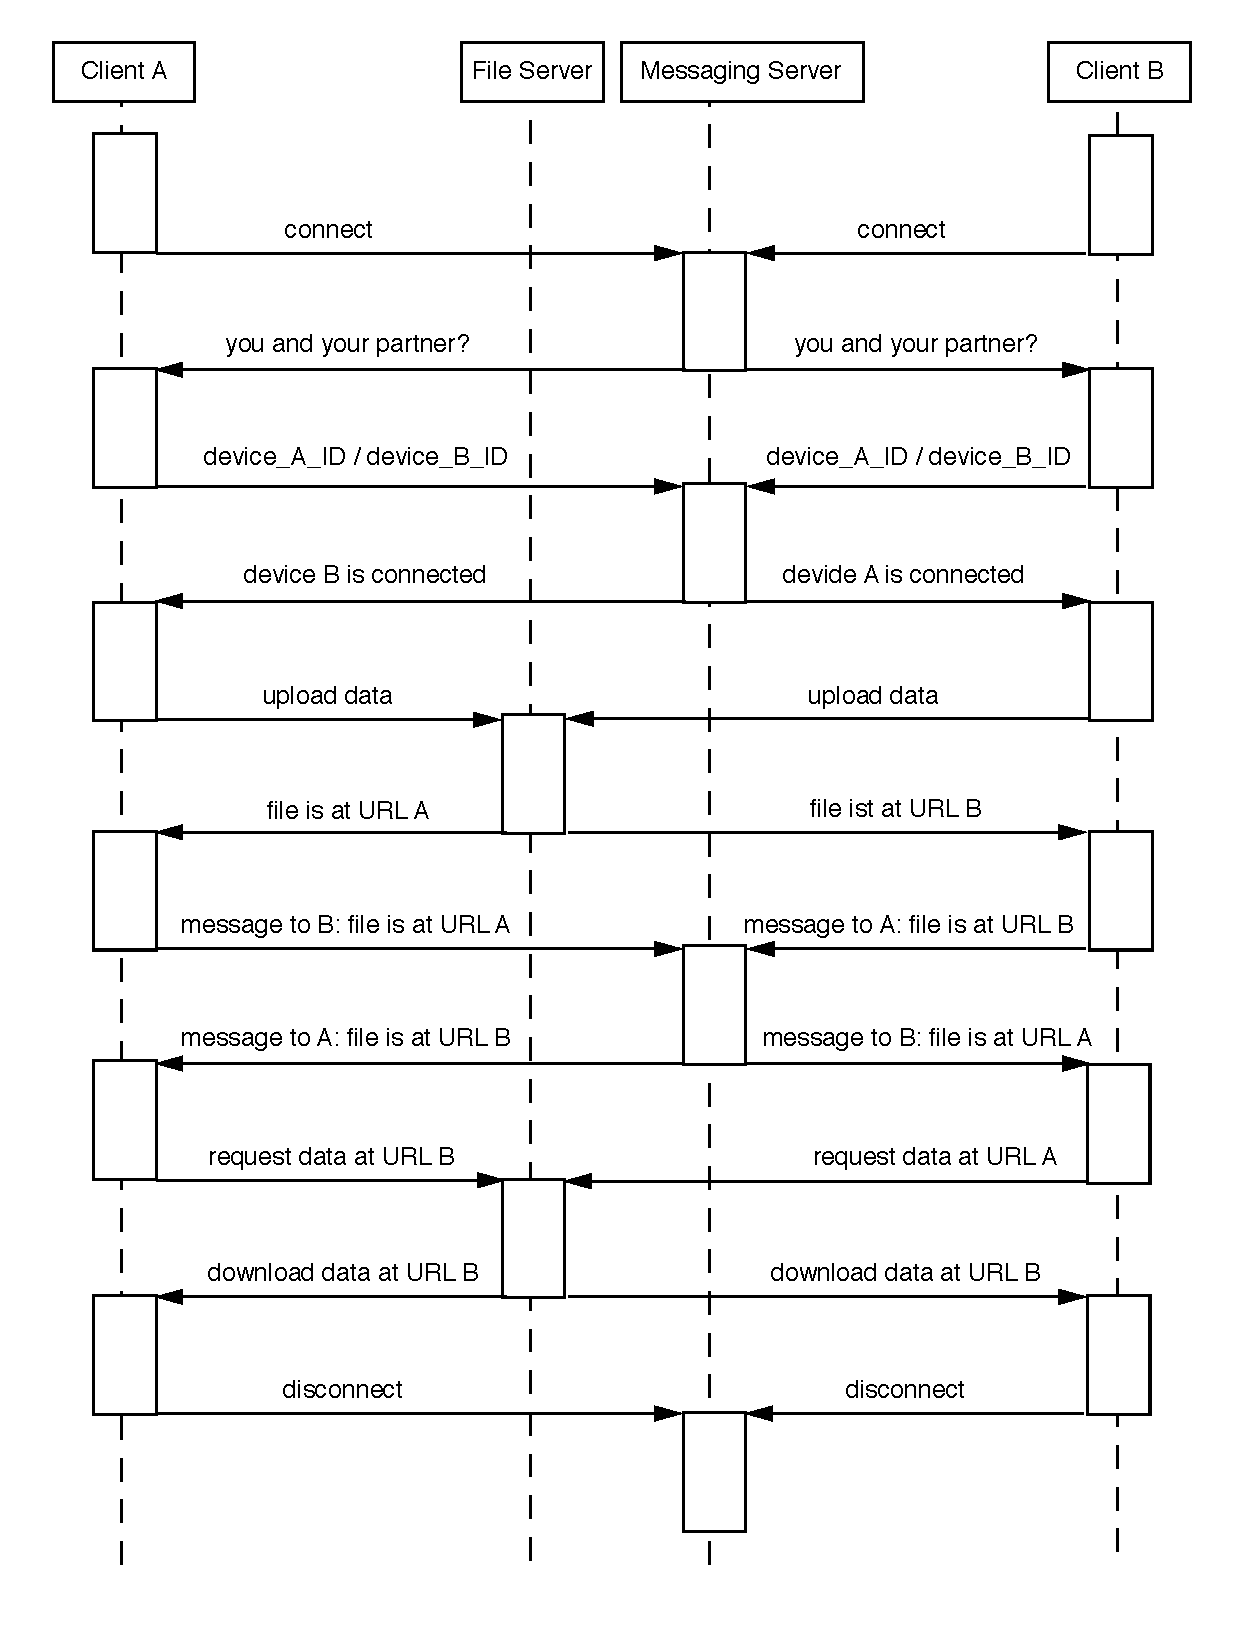
\includegraphics[width=\linewidth]{kapitel4/umlServer.pdf}
    \caption{Sequenzdiagramm Datenaustausch über Webserver}
    \label{fig:sequenz}
\end{figure}

\newpage
\subsection{Vergleich der Konzepte}
\label{sec:Systemvergleich}
Direkte Kommunikation bietet den Vorteil, ohne zusätzliche Server Infrastruktur zu operieren und es wird, falls der Server nur über das Internet erreichbar ist, auch keine Internetverbindung benötigt. Nachteilig ist jedoch der höhere Implementierungsaufwand, um für jede Plattform ein System anzubieten. Die von den Plattformen genutzten Technologien und Frameworks sind teilweise nicht kompatibel, was es erforderlich macht, für jede Plattform Einzellösungen zu implementieren. Wird dagegen eine Serverarchitektur gewählt, ist der Implementierungsaufwand wesentlich geringer, da die meiste Implementierung nur einmal für den Server erfolgen muss. Nachteilig ist der erforderliche Zugang zu entweder einem lokalen \ac{WLAN} oder zu mobilem Internet. Weiterhin handelt es sich bei einem Server um einen Single-Point-Of-Failure. Fällt der Server aus, funktioniert das komplette System nicht mehr. Hier bieten lokale Lösungen einen klaren Vorteil, da diese ausfallsicher sind. Weiterhin ist der Betrieb eines Servers auch mit Kosten verbunden die in einem lokalen System nicht anfallen.